	Pour ce projet, nous avons décider d'installer Windows Server 2003 Entreprise Edition, afin d'avoir un sytème d'exploitation récent. Toutes les fonctionnalités utilisées pour la création d'un VPN sont incluses dans cette version. Il n'y a pas besoin d'installer une application tierce.
	Voyons à présent les différents services nécessaires pour la mise en place du VPN de Microsoft.

\subsubsection{Services installés}

	Afin de pouvoir se mettre dans les conditions du réseau interne de l'ISIMA, nous avons décidé de configurer plusieurs services:
~


\begin{itemize}
	\item  - DHCP,
	\item  - DNS, 
	\item  - Active Directory,
	\item  - Routage et accès distant.(VPN)
\end{itemize}
~	

	Ces nombreux services sont nécessaires pour la création d'un VPN. A présent, détaillons la configuration de chacun de ces servives. 
	Remarque : Sous windows on ne parle pas de serveur mais de service. Tout les fonctionnalités de la machine (DNS, DHCP ou autre) sont référencés comme des services.


\paragraph{Caractéristique de la machine}
~\

Le serveur windows est installé sur un DELL PowerEdge 1300. Il est doté d'un processeur INTEL de type Pentium II cadencé à 348 Mhz. Il possède 512 Mo de mémoire vive et un disque dur de 9 Go.
Le serveur est composé de trois cartes réseaux, une pour le réseau extérieur et deux autres pour le réseau interne. 



Voici leur adresse IP:

\begin{figure}[H]
	\begin{center}
\begin{tabular}{|l|c|c|}
\hline
Caractéristique & Réseau & Adresse IP \\
\hline
Realtek RTL 8139 Familly & réseau PROFS & 10.0.0.11/24 \\
Realtek RTL 8139 Familly & réseau extérieur & 192.168.102.250/24 \\
Fast Ethernet CNET PRO 200P & réseau STUDENTS & 192.168.0.11/24 \\
\hline
\end{tabular}
	\end{center}
	\caption{Caractéristique des cartes réseaux}
	\label{IP_carte_reseau}
\end{figure}

Tout les cartes installés sont de type 100Mbit/s.
~

\paragraph{Service DHCP}
~\


Ce service est nécessaire pour l'attribution des adresses IP qui seront allouées aux différents clients lors de leurs connexion au serveur VPN. Nous avons configurer le service DHCP de la manière suivante. Sachant que le serveur VPN doit avoir deux cartes réseaux indépendantes (une sur le réseau STUDENTS et une sur le réseau PROFS) le DHCP peut fournir deux pools d'adresse différents. 
Voici les caractéristiques des deux réseaux:

\begin{figure}[H]
	\begin{center}
\begin{tabular}{|l|c|c|}
\hline
Caractéristique & Réseau PROFS & Réseau STUDENTS \\
\hline
Désignation Carte réseau & DHCP\_PROFS & DHCP\_STUDENTS \\
Adresse IP Carte réseau & 10.0.0.11 & 192.168.0.11 \\
Pool d'adresse & 10.0.2.100 à 10.0.2.254 & 192.168.0.100 à 192.168.0.254 \\
Masque réseau & 255.255.255.0 & 255.255.255.0 \\
Serveur DNS/routeur & 10.0.0.11 & 192.168.0.11 \\
Nom du domaine DNS & wvpn.isima.fr & wvpn.isima.fr \\
\hline
\end{tabular}
	\end{center}
	\caption{Caractéristique du service DHCP}
	\label{service_DHCP}
\end{figure}

Il est à noter que lors de l'installation du service DHCP, et en dehors des différentes configurations des cartes, il n'y a pas d'options spécifiques. Ce sont les options par défaut.
Il est à remarquer que le service DHCP se compose de deux étendues, une pour chaque carte. Cependant, le service DHCP s'attache à une seule carte réseau et non au deux. Dans la maquette, le service se lie avec la carte DHCP\_PROFS. Pour illustrer ces propos, voici un screenshot du service DHCP.

\begin{figure}[H]
	\begin{center}
	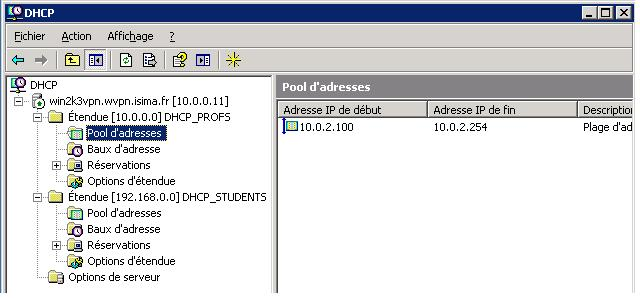
\includegraphics[width=\textwidth]{partie_2/screen_windows/dhcp.JPG}\\
	\end{center}
	\caption{Lien avec la carte réseau DHCP\_PROFS}
	\label{Screen_client_dhcp}
\end{figure}


On remarque que bien que la présence des deux étendues et que la carte DHCP\_PROFS (10.0.0.11) s'attache au service DHCP.
~\


Voyons à présent la configuration du service DNS.

\paragraph{Service DNS}
~\


Afin de pouvoir utiliser l'active directory nous avons du installer ce service. Celui-ci nous permet de résoudre les différentes adresses IP qui seront nécessaire lorsq'un client VPN se connectera sur le réseau interne.
Voici les caractèristiques du service DNS:
~\


\begin{figure}[H]
	\begin{center}
\begin{tabular}{|l|c|c|}
\hline
Caractéristique & Serveur Windows2003 \\
\hline
Nom de la machine &  win2k3vpn\\
Nom du domaine & wvpn.isima.fr\\
Type de zone &  zone principale\\
\hline
\end{tabular}
	\end{center}
	\caption{Caractéristique du service DNS}
	\label{service_DNS}
\end{figure}

~\

Il est à remarquer que lors de l'installation du service, nous avons décider d'incorporer la zone de recherche inversée. Le serveur windows étant composé de trois cartes réseaux, il y a trois zones. Afin de vérifier que le service DNS est bien configurer, la commande NSLOOKUP nous permet de tester le DNS. 
L'illustration suivante montre la résolution DNS est correcte.

\begin{figure}[H]
	\begin{center}
		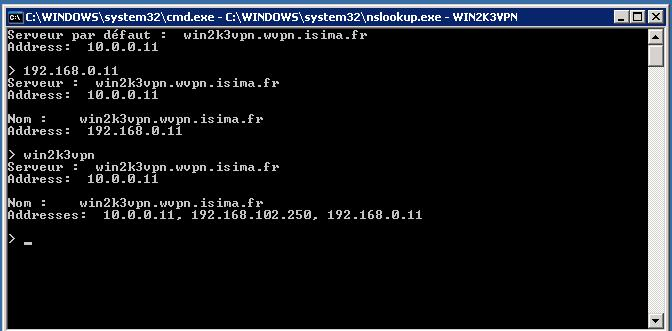
\includegraphics[width=\textwidth]{partie_2/screen_windows/nslookup.JPG}\\
	\end{center}
	\caption{Résolution DNS}
	\label{NSLOOKUP}
\end{figure}

Tout comme le service DHCP, le service DNS se lie avec une seule carte réseau. 

Intéressons nous à présent à la configuration de l'Active Directory.

\paragraph{Active Directory}
~\

Ce service nous a permi de créer un annuaire afin d'indentifier les clients souhaitant se connecter sur le réseau interne.